\begin{figure}[tbhp]
  \centering
  \subfigure[GN Exp 11, \textsc{CTEvent} Size = 10 Num.Slot = 100]{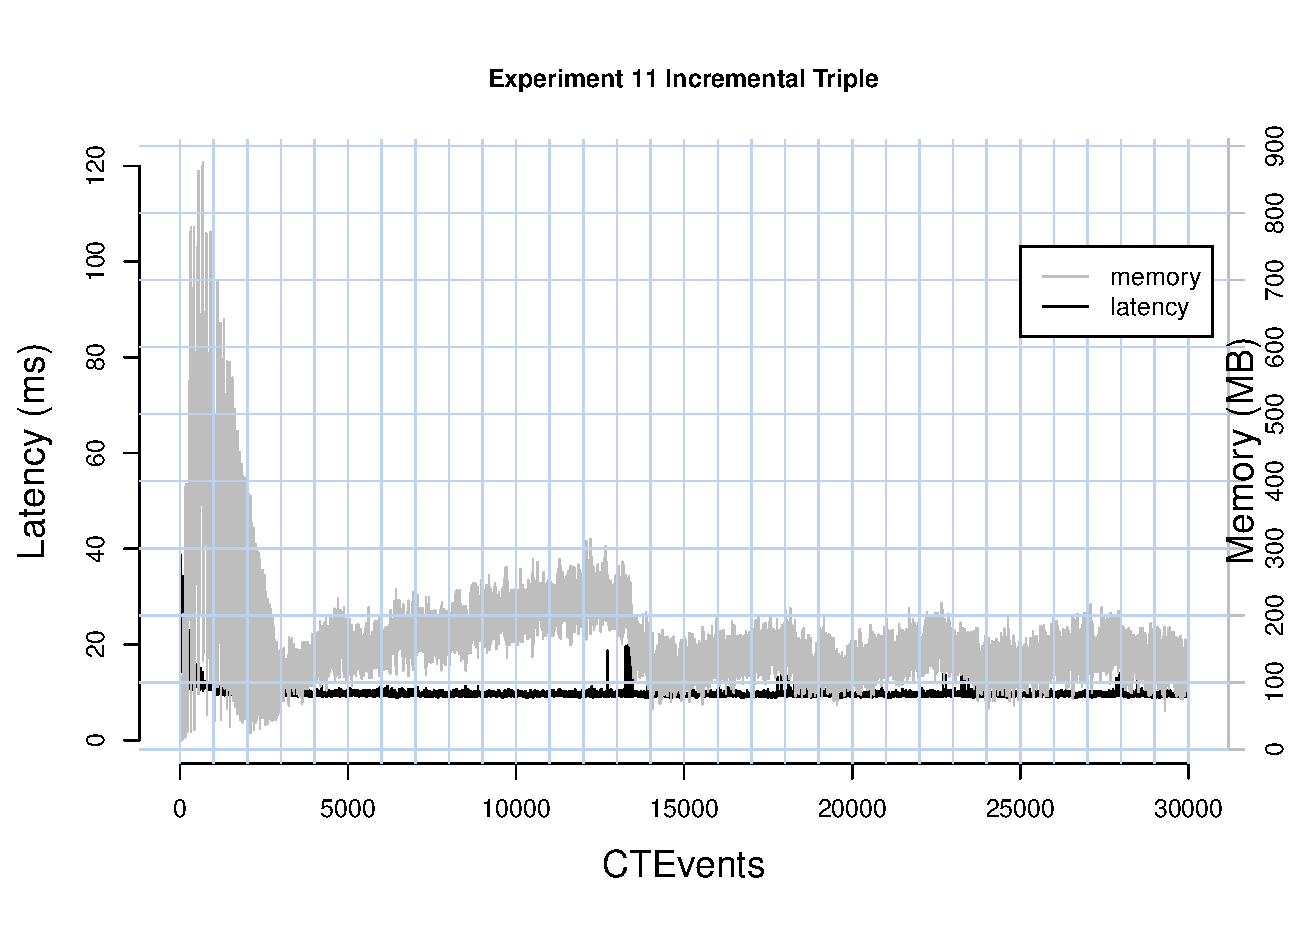
\includegraphics[width=\linewidth]{images/level3-not-steady-naive-graph-en11}}
  \subfigure[TI Exp 11, \textsc{CTEvent} Size = 10 Num.Slot = 100]{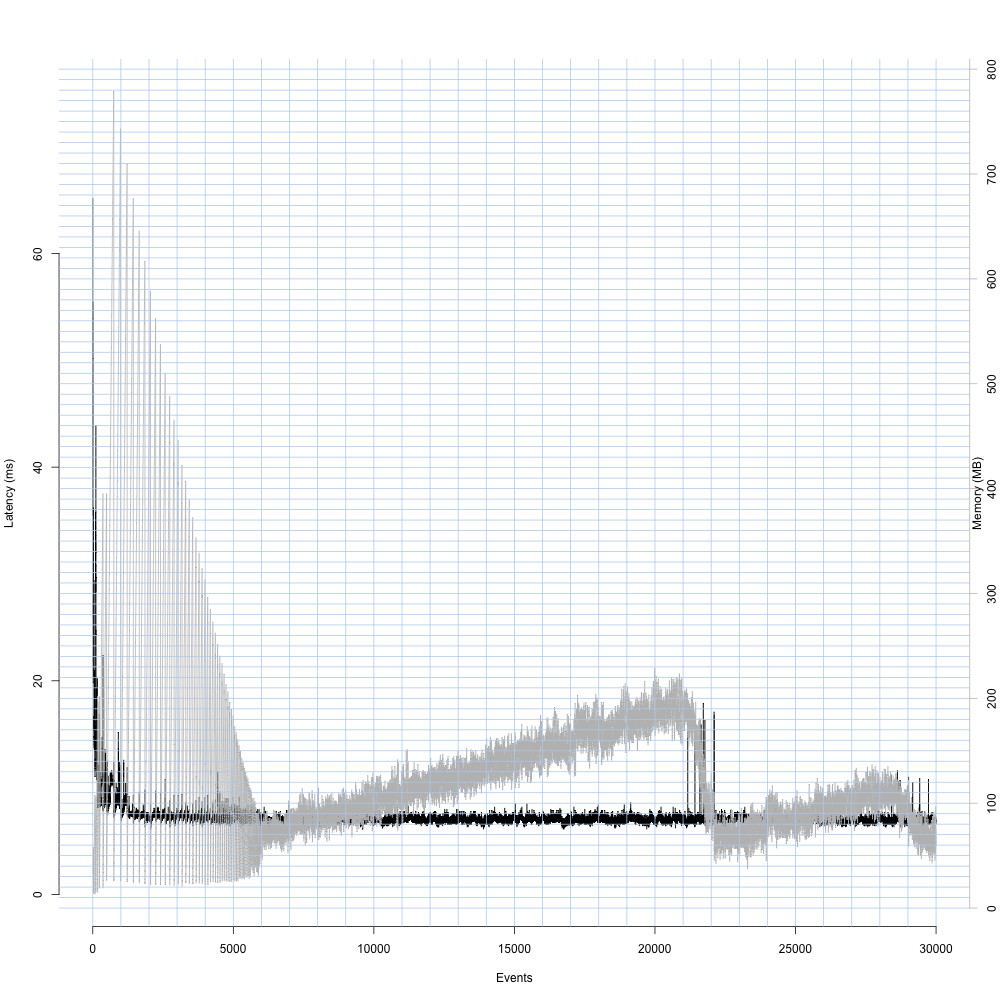
\includegraphics[width=\linewidth]{images/level3-not-steady-inc-stmt-en11}}
  \caption[\textsc{Analyser} Investigation Stack - Level 3 - Intra Experiment Comparison - SOAK Test Latency vs Memory Not Steady State Reaching]{Comparison between memory and latency on difference in Steady State condition reaching} 
  \label{fig:level3-not-steady-naive-graph-en11}
\end{figure}

\begin{figure}[tbph]
  \centering
  \subfigure[GN Exp 7, \textsc{CTEvent} Size = 10, Num.Slot = 10]{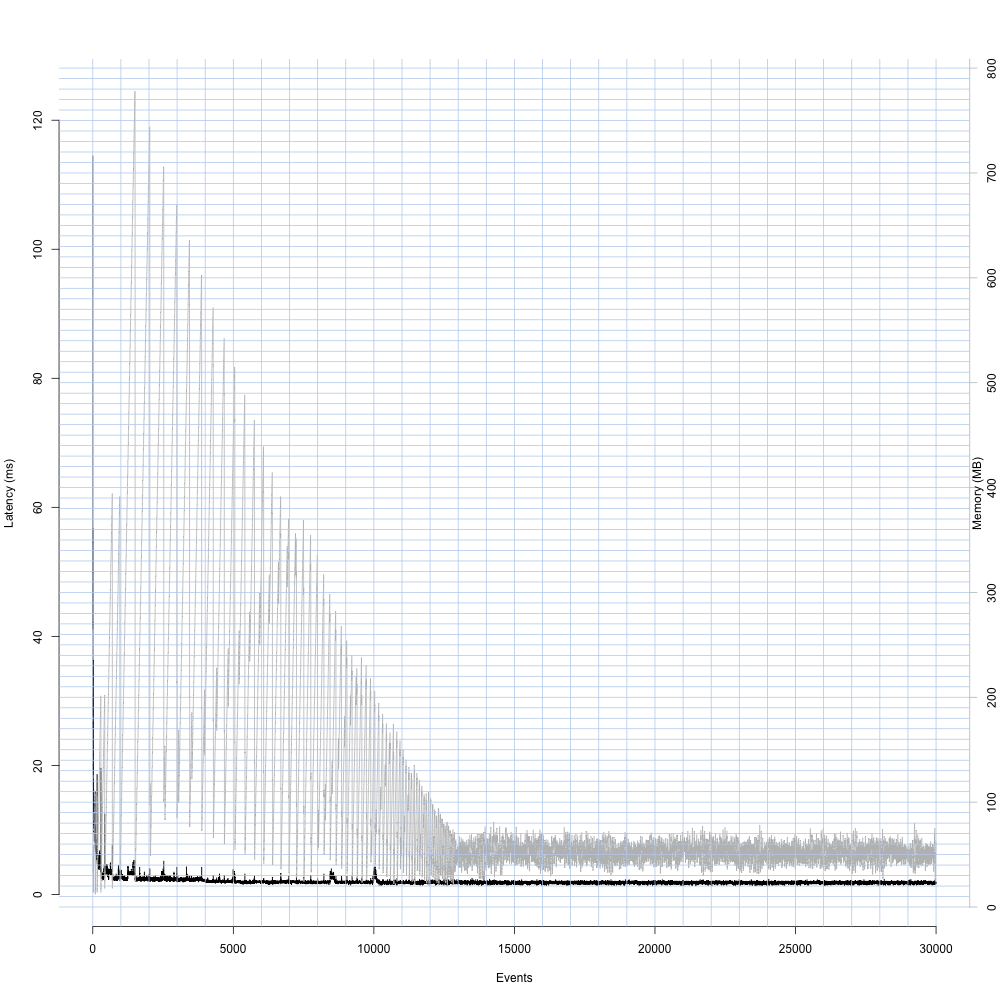
\includegraphics[width=\linewidth]{images/level3-steady-naive-graph-en7}}
   \subfigure[GI Exp 12, \textsc{CTEvent} Size = 100, Num.Slot = 100]{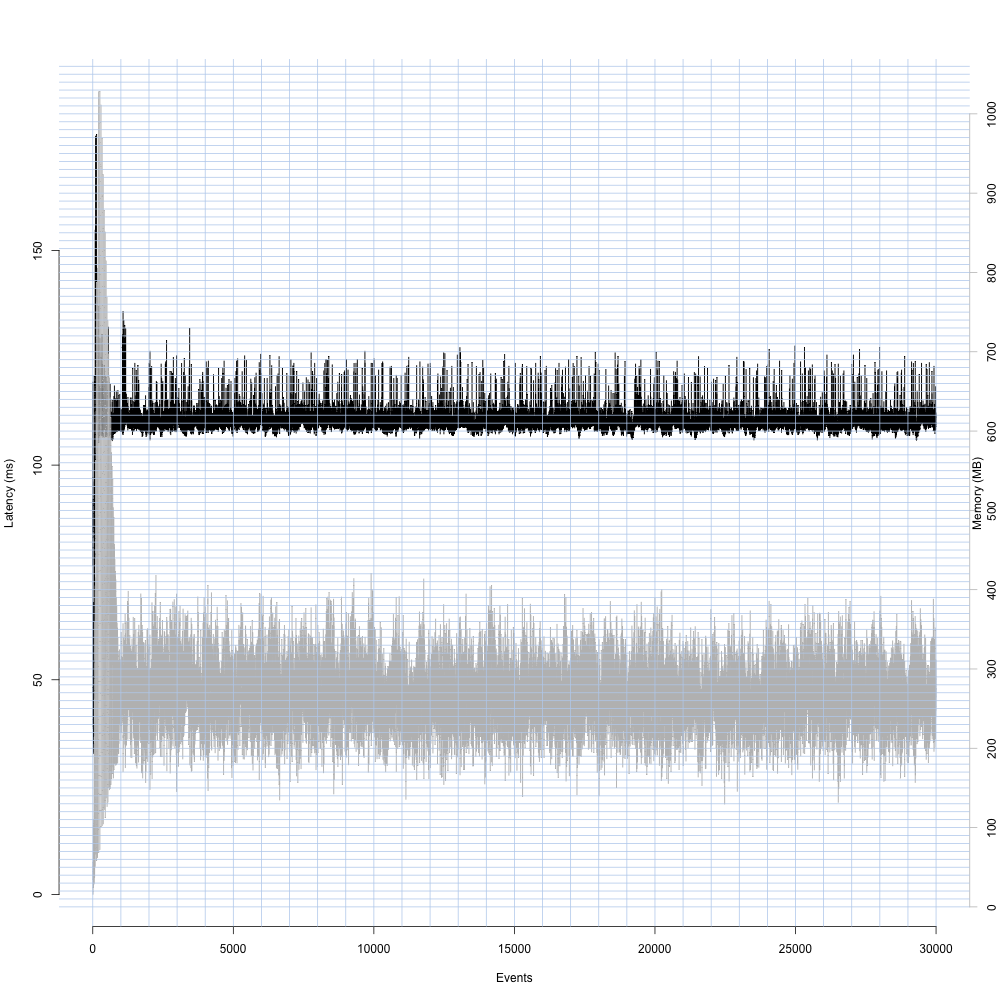
\includegraphics[width=\linewidth]{images/level3-steady-inc-graph-en12}}
  	\caption[\textsc{Analyser} Investigation Stack - Level 3 - Intra Experiment Comparison - SOAK Test Latency vs Memory Steady State Reaching]{Comparison of steady state condition reaching between latency and memory}
  	\label{fig:level3-steady-naive-graph-en12-7}  	
\end{figure}

\begin{figure}[tbph]
  \centering
  \subfigure[TN Exp 15, \textsc{CTEvent} Size = 1 Num.Slot = 10000]{
	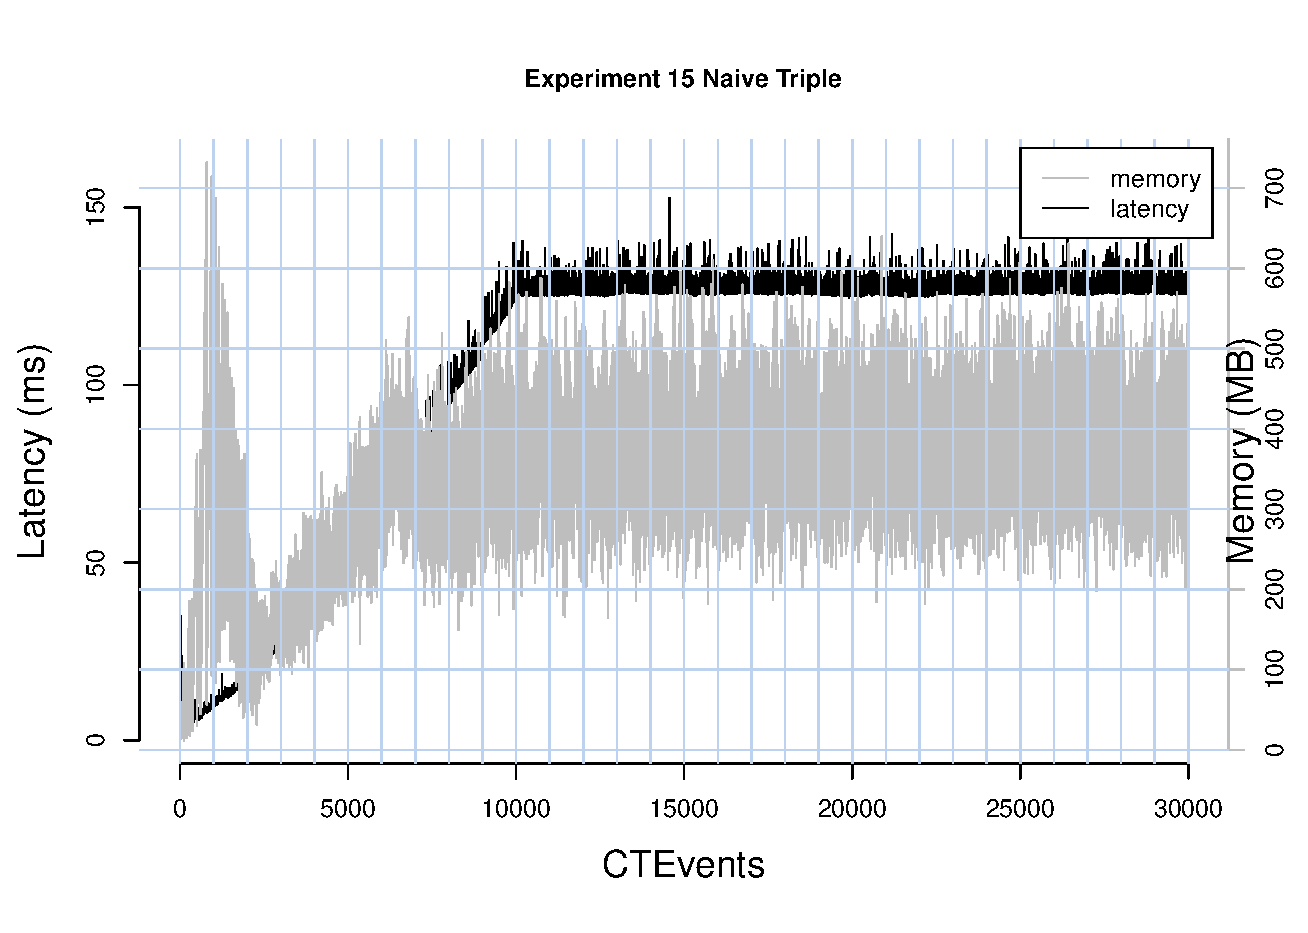
\includegraphics[width=\linewidth]{images/level3-filling-naive-stmt-en15}
	}
\subfigure[TI Exp 15, \textsc{CTEvent} Size = 1 Num.Slot = 10000]{
	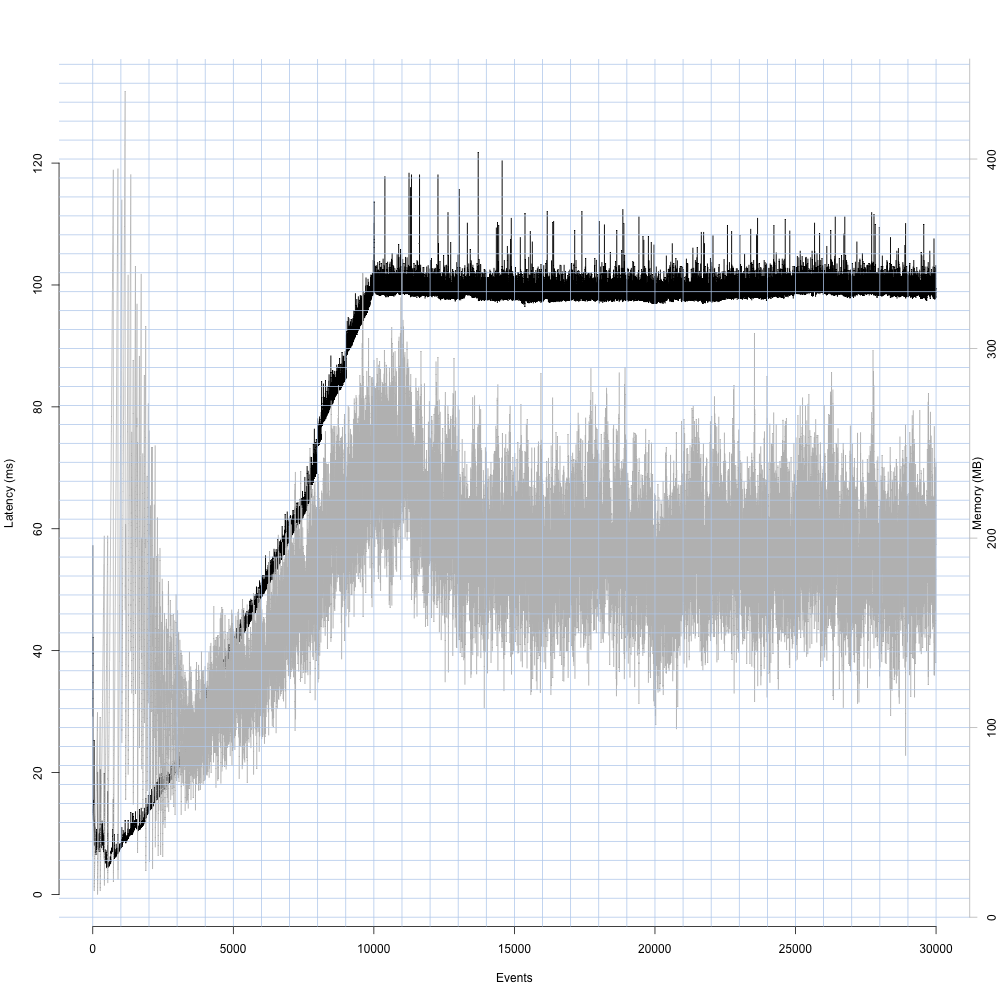
\includegraphics[width=\linewidth]{images/level3-filling-inc-stmt-en15}
	}
	\caption[\textsc{Analyser} Investigation Stack - Level 3 - Intra Experiment Comparison - SOAK Test Latency vs Memory Filling Phenomena]{Comparison of filling phenomena between latency and memory} 
  	\label{fig:level3-filling-inc-stmt-en15}
\end{figure}